\begin{frame}{Motivation --- Galloping Horses}
  \begin{center}
    ``Sallie Gardner at a Gallop'' --- Eadweard Muybridge
    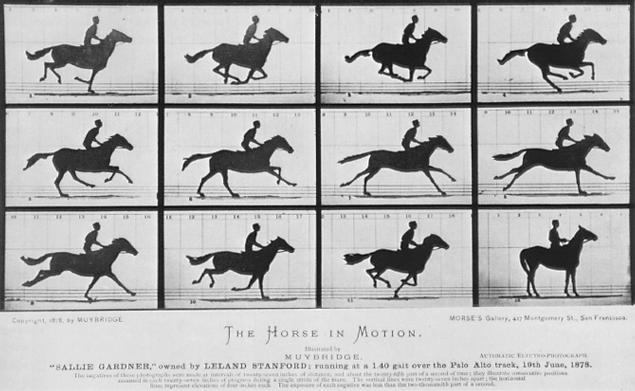
\includegraphics[width=0.75\linewidth]{muybridge_galloping_horse}
  \end{center}
\end{frame}

\begin{frame}{Modern ``Galloping Horses''}
  \begin{center}
    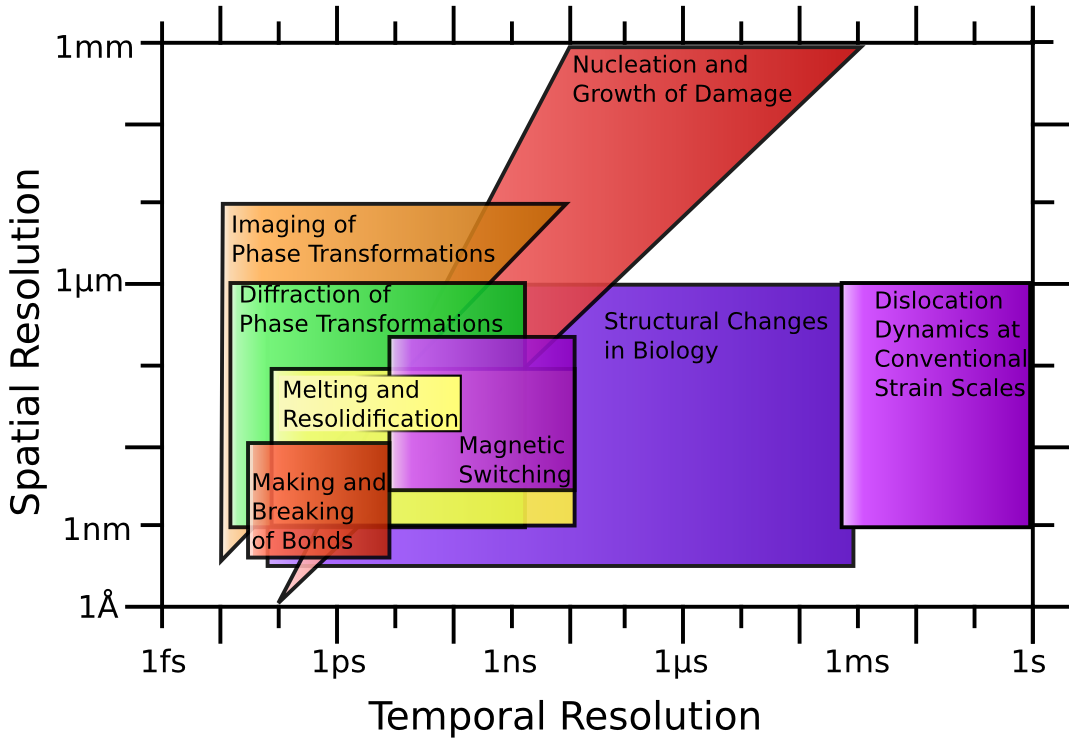
\includegraphics[width=0.85\linewidth]{Resolution}
  \end{center}
\end{frame}

\begin{frame}{Resolutions of TEM and Lasers}
  \begin{columns}	
    \begin{column}{0.49\linewidth}
      Transmission Electron Microscopy (TEM) resolution:
      \begin{itemize}
        \item<2-> JEOL 2010F: 0.19nm
        \item<3-> FEI Titan G2: 0.08nm
        \item<4-> TEAM aberration corrected microscope aims for 0.05nm
        \item<5-> Temporal resolution: video rate (commonly $\sim$30fps)
      \end{itemize}
      \begin{figure}
        \centering
        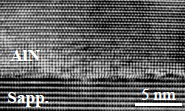
\includegraphics{hrtem}
        \caption{\url{le-csss.asu.edu}}
      \end{figure}
    \end{column}
    \begin{column}{0.49\linewidth}
      Laser resolution:
      \begin{itemize}
        \item<6-> Ultrafast Lasers
        \begin{itemize}
          \item<7-> Ti:Sapphire $\sim 10$fs 
          \item<8-> As short as 80 attosecond
          \item<9-> Limited by optical wavelength
        \end{itemize}
        \item<10-> Near field scanning optical microscopy (NSOM)
        \begin{itemize}
          \item<10-> Uses sub-wavelength apertures
          \item<10-> 2-5nm resolution
          \item<10-> Long scan time
        \end{itemize}
      \end{itemize}
      \begin{figure}
        \centering
        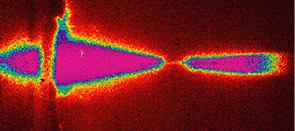
\includegraphics{channel}
        \caption{\url{www.xrimlab.com}}
      \end{figure}
    \end{column}
  \end{columns}
\end{frame}

\begin{frame}{Laser Driven Time-Resolved Electron Microscope}
  \begin{center}
    \begin{tikzpicture}
      \node {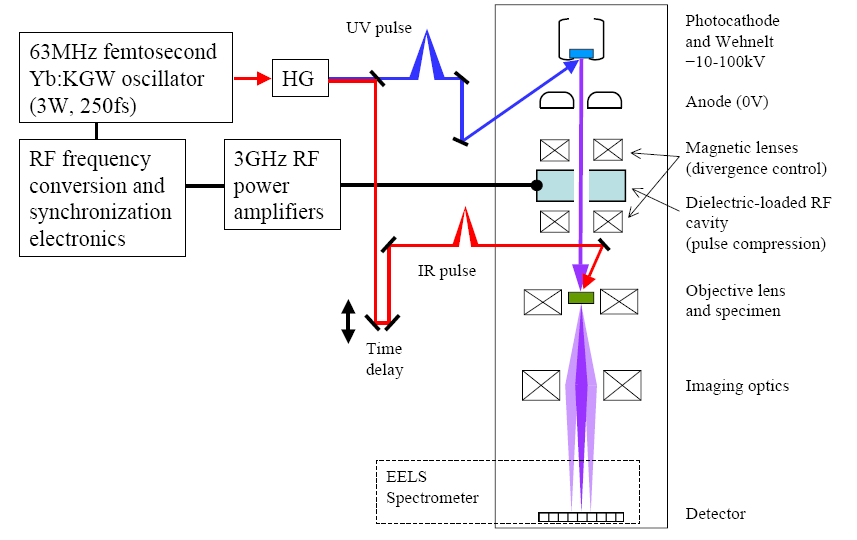
\includegraphics[width=0.85\linewidth]{UEM}};
      \node at (-3,-2) [text width=5cm] {
        \begin{itemize}
          \item<2-> Time-Integrated
          \item<3-> Stroboscopic
          \item<4-> Single-Shot
        \end{itemize}
      };
    \end{tikzpicture}
  \end{center}
\end{frame}

% added modes to above
%\begin{frame}{Operational Modes}
%  Along with the usual TEM modes of operation
%  \begin{itemize}
%    \item Imaging
%    \item Diffraction
%    \item HAADF
%    \item EELS
%    \item etc.
%  \end{itemize}
%  \uncover<2->{TR-EM offers an additional mode choice}
%  \begin{itemize}
%    \item<3-> Single-Shot (assumed mode for this talk)
%    \item<4-> Stroboscopic (requires repeatable process)
%    \item<5-> Time-integrated (Conventional operation)
%  \end{itemize}
%\end{frame}

\begin{frame}{Instruments in Development}
\begin{center}
\begin{tikzpicture}
  \node (image) {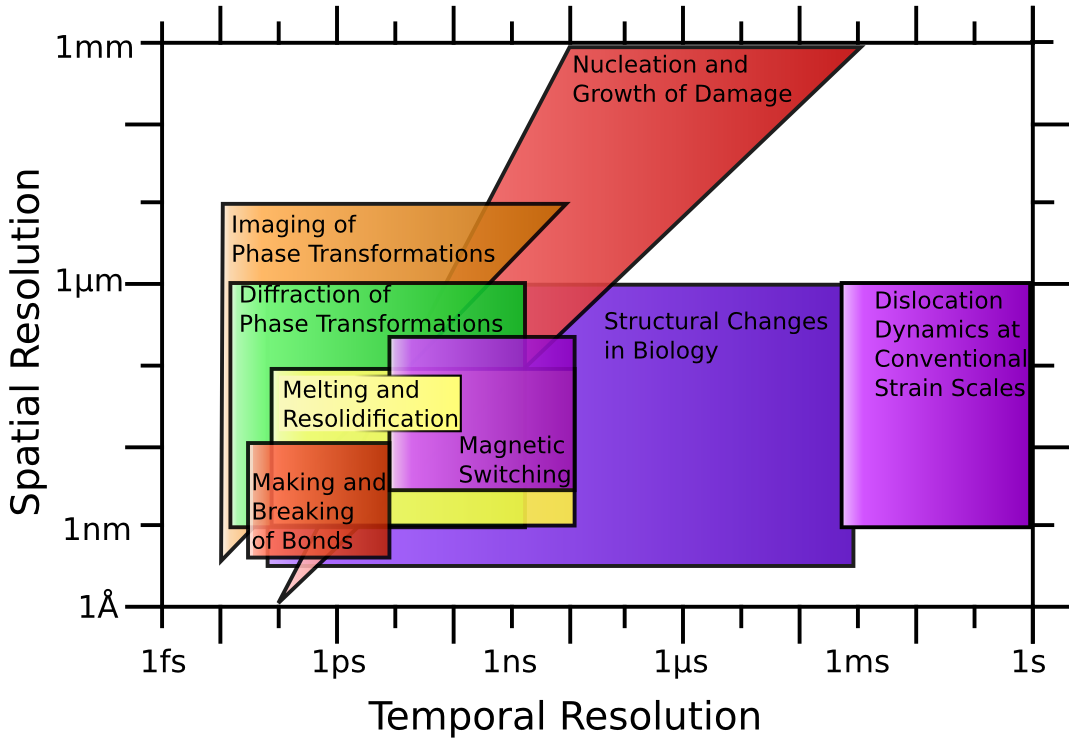
\includegraphics[width=0.7\linewidth]{Resolution}};
  \visible<2->{
    \node [
      star,
      star point ratio = 2,
      inner sep = 0.7mm,
      draw,
      fill=white,
      pin={[draw,fill=white,pin edge=thick] above:{\tiny TU-Berlin}}
    ] at (0.3,0.1) {};
    \node [
      star,
      star point ratio = 2,
      inner sep = 0.7mm,
      draw,
      fill=white,
      pin={[draw,fill=white,pin edge=thick] right:{\tiny UEM-2 Caltech}}
    ] at (0.3,-0.3) {};
    \node [
      star,
      star point ratio = 2,
      inner sep = 0.7mm,
      draw,
      fill=white,
      pin={[draw,fill=white,pin edge=thick,pin distance=0.6in] above:{\tiny Caltech stroboscopic}}
    ] at (-1.3,-0.3) {};
    \node [
      star,
      star point ratio = 2,
      inner sep = 0.7mm,
      draw,
      fill=white,
      pin={[draw,fill=white,pin edge=thick] right:{\tiny LLNL}}
    ] at (0.4,-0.6) {};
    \node [
      star,
      star point ratio = 2,
      inner sep = 0.7mm,
      draw,
      fill=white,
      pin={[draw,fill=white,pin edge=thick] right:{\tiny UC-Davis Bio-DTEM}}
    ] at (1.2,-1.1) {};
  }
  \end{tikzpicture}
  \end{center}
\end{frame}
